\documentclass[a4paper]{article}
\title{MAT257---Analysis 2}
\author{Jonah Chen}

\usepackage[utf8]{inputenc}
\usepackage[margin=0.5in]{geometry}

\usepackage{braket}
\usepackage{physoly}
\usepackage{currfile}
\usepackage{gensymb}
\usepackage{amssymb}
\usepackage{pgf,tikz,pgfplots}
\usepackage{mathrsfs}
\usepackage{textcomp}\usepackage{accents}
\newcommand{\ubar}[1]{\underaccent{\bar}{#1}}

\usetikzlibrary{arrows}
\numberwithin{equation}{section}
\pgfplotsset{compat=1.16}
\everymath{\displaystyle}

\newcommand{\R}{\mathbb{R}}
\newcommand{\Z}{\mathbb{Z}}
\newcommand{\vol}{\mathrm{vol}}
\begin{document}
\sffamily
\maketitle
\tableofcontents
\section{Course Overview}
\begin{itemize}
    \item $\mathbb R\to\mathbb R^n$
    \item Linear Algebra
    \item Continuity
    \item Differentiability
    \item Integration
    \item Key theorem of this class is \textbf{Stokes' Theorem}
    \begin{equation}
        \int_C\dd\omega=\int_{\partial C}\omega
    \end{equation}
    Generalizes the fundamental theorem of calculus:
    \begin{equation}
        \int_{[a,b]}F'(t)\dd t=F(b)-F(a)=\int_{\partial[a,b]}F
    \end{equation}
    Note that $\partial[a,b]=\{b+, a-\}$.
\end{itemize}

\section{Distances}
\begin{itemize}
    \item Roughly speaking, continuity from $\mathbb R\to\mathbb R$ means if two points are near, their images should be near also.
    \item Thus, in $\mathbb R^n$, the intuitive meaning should be similar.
\end{itemize}
\subsection{Norms and Inner Product}
Note there are 2 conventions for $\mathbb R^n$
\begin{enumerate}
    \item The set of all n-dimensional real column vectors.
    \item The set of all n-dimensional real row vectors.
\end{enumerate}
In this class, the distinction is not very important.

\begin{definition}
    For $x, y\in\mathbb R^n$, "The standard (or euclidian) inner product of $x$ and $y$, denoted 
    \begin{equation}
        \langle x, y\rangle = \sum_{i=1}^n x_iy_i
    \end{equation}
    The norm-squared of $x$ is 
    \begin{equation}
        |x|^2=\langle x, x\rangle = \sum x_i^2
    \end{equation}
    and the norm of $x$ is
    \begin{equation}
        |x|=\sqrt{|x|^2} = \sqrt{\sum x_i^2}
    \end{equation}
\end{definition}

\begin{proposition}
    If $x, y, z\in\mathbb R^n$ and $a, b\in\mathbb R$, then
    \begin{enumerate}
        \setcounter{enumi}{-1}
        \item The inner product is bilinear \& the norm is ``semi-linear''.
        \begin{align}
                \langle ax+by,z \rangle &= a\langle x, z\rangle + b\langle y, z\rangle\\
            \langle z, ax+by \rangle &= \dots\\
            |ax|&=|a||x|
        \end{align}
        \textbf{Aside}: 
        \begin{equation}
            1=\sqrt 1=\sqrt{-1\cdot-1}=\sqrt{-1}\sqrt{-1}=i\cdot i=-1
        \end{equation}
        \item \begin{equation}
            |x|\geq 0 \& |x|=0\iff x=0
        \end{equation}
        \item \begin{equation}
            \langle x,y\rangle = \langle y,x \rangle
        \end{equation}
        \item \textit{Cauchy-Schwarz inequality}
        \begin{equation}
            |\langle x,y\rangle|\leq|x||y|
        \end{equation}
        with equality if $x\&y$ are dependent. 
        \item \textit{Triangle inequality}
        \begin{equation}
            |x+y|\leq |x|+|y|
        \end{equation}
        \item \textit{Polarization identity}
        \begin{equation}
            \langle x,y\rangle = \frac{|x+y|^2-|x-y|^2}{4}
        \end{equation}
    \end{enumerate}

    \begin{proof}
        \begin{enumerate}
            \item $|x|=\sqrt{\sum x_i^2}$
            $|x|=0\implies\sum x_i^2=0\implies\forall i, x_i^2=0\implies \forall i,x_i=0\implies x=0$
            \item 
            For $s,t\in\mathbb R^n$
            \begin{equation}
                |s+t|^2=|s|^2+|t|^2+2\langle s,t \rangle
            \end{equation}
    
            Look at 
            \begin{align}
                0\leq\Big||y|^2x-\langle x,y\rangle y\Big|^2&=|y|^4|x|+\langle x,y\rangle^2|y|^2-2|y|^2\langle x,y\rangle^2\\
                &=|y|^2\left(|y|^2|x|^2-\langle x,y \rangle^2\right)
            \end{align}
            This is equal to zero only if $|y|^2x-\langle x,y\rangle y=0$. If we have equality, that implies $x\&y$ are dependent.
            \\\textbf{Why, what does this mean?}
            \item 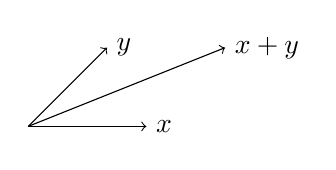
\begin{tikzpicture}
                \draw[->] (0,0) -- (1,1)node[anchor=west]{$y$};
                \draw[->] (0,0) -- (1.5, 0) node[anchor=west]{$x$};
                \draw[->] (0,0) -- (2.5, 1)node[anchor=west]{$x+y$};
            \end{tikzpicture}
            As both sides of the triangle inequality are $\geq0$, square both sides.
            \begin{align}
                |x+y|^2&\stackrel{?}{\leq}(|x|+|y|)^2\\
                \langle x+y, x+y \rangle&\stackrel{?}{\leq}|x|^2+|y|^2+2|x||y|\\
                \langle x,x\rangle + 2\langle x,y\rangle + \langle y,y\rangle &\stackrel{?}{\leq}|x|^2+|y|^2+2|x||y|\\
                |x|^2+|y|^2+2\langle x,y\rangle &\stackrel{?}{\leq}|x|^2+|y|^2+2|x||y|\\
                \langle x,y\rangle &\stackrel{?}{\leq}|x||y|\label{220}
            \end{align}
            \eqref{220} is true by cauchy-schwarz.
            \item The proof is trivial because you can expand the right hand side.
            \\\textbf{Note:} The inner product and the norm are not independent. If you know how to compute one, you can compute the other.
        \end{enumerate}
    \end{proof}
\end{proposition}
\subsection{Distance Functions}
\begin{definition}
    If $x, y\in\R^n$,define the distance between $x\&y$
    \begin{equation}
        d(x,y)=|x-y|
    \end{equation}
\end{definition}
\begin{theorem}
    \begin{enumerate}
        \item $d$ is symmetric: $d(x,y)=d(y,x)$
        \item $d$ is positive definite: $d(x,y)\geq0$ and $d(x,y)=0\iff x=y$
        \item Triangle inequality: $d(x,z)\leq d(x,y)+d(y,z)$
    \end{enumerate}
    The significance of this theorem is that this is all we need to know about distances to comment on continuity.\\
    \textbf{Aside:} Later, this theorem will become a definition for a distance function or a metric.
    \begin{proof}
        \begin{enumerate}
            \item \begin{align}
                d(x,y)=|x-y|=|-(y-x)|=|-1||y-x|=|y-x|=d(y,x)
            \end{align}
            \item \begin{align}
                d(x,y)=0\iff |x-y|=0\iff x-y=0\iff x=y
            \end{align}
            \item \begin{align}
                |x-z|\stackrel{?}{\leq}|x-y|+|y-z|
            \end{align}
            This is true by the previous triangle inequality, $|p|+|q|\geq|p+q|$. Letting $p=x-y,q=y-z\implies p+q=x-z$.
        \end{enumerate}
    \end{proof}

    There are other norms and distance functions that we will rarely use.

    \begin{itemize}
        \item The euclidian norm which we use is $|x|_{L^2}=\sqrt{\sum x_i^2}$.
        \item There is a L1 norm $|x|_{L^1}=\sum|x_i|$.
        \item The L-infinity norm is $|x|_{L^\infty}=\max |x_i|$.
    \end{itemize}
    The distance functions for these norms also satisfys these three properties.
\end{theorem}

\begin{itemize}
    \item There is a bijection between linear maps from $\R^n\to\R^m$ and the set of $m\times n$ matrices with real coefficients. This bijection can be realized by choosing a basis. 
    \item In $\R^n$ or $\R^m$, there is a natural basis (the standard basis) $e_i=\begin{pmatrix}
        0\\
        \vdots\\
        1\\
        \vdots\\
        0
    \end{pmatrix}\leftarrow i-$th position
    \item by $A\in M_{m\times n}\to L_A(x)=Ax$, where $x\in\R^n$.
    \item If T is a linear transformation, $M_T=\begin{pmatrix}\:\\
        Te_1|Te_2|\dots|Te_n\\\:
    \end{pmatrix}$
\end{itemize}
\begin{definition}
    Homomorphism: A map that preserve the structure.
\end{definition}
\begin{theorem}
    \begin{enumerate}
        \setcounter{enumi}{-1}
        \item Bijective
        \begin{align}
            L_{(M_T)}=T, M_{(L_A)}=A
        \end{align}
        \item \begin{itemize}
            \item $A\to L_A$ is linear: $L_{aA+bB}=aL_A+bL_b$
            \item $T\to M_T$ is linear: $M_{aT+bS}=aM_T+bM_S$
        \end{itemize}
        \item Given $T: \R^n\to\R^m, S:\R^m\to\R^p$, and $S\circ T\equiv T//S: \R^n\to\R^p$.\\
        Then, $M_SM_T=M_{S\circ T}$.
    \end{enumerate}
\end{theorem}

End of the review.

\section{Rectangles}
\begin{itemize}
    \item It is common to use intervals in $\R$. In $\R^n$, we use rectangles. 
    \item To specify a rectangle, we must bound the each of the $n$ coordinates.
\end{itemize}
\begin{definition}
    Given $a_i\leq b_i$, where $i=1,\dots, n$,
    \begin{itemize}
        \item The closed rectangle corresponding to $a_i,b_i$ is defined as
        \begin{align}
            R=\prod_{i=1}^n[a_i,b_i]=\{x\in\R^n:\forall i\:\: a_i\leq x_i\leq b_i\}
        \end{align}
        \item The opened rectangle defined by $a_i,b_i$ is defined as 
        \begin{align}
            R=\prod_{i=1}^n(a_i,b_i)=\{x\in\R^n:\forall i\:\: a_i<x_i<b_i\}
        \end{align}
    \end{itemize}
\end{definition}
\begin{itemize}
    \item If $X\&Y$ are sets, we define (from set theory) the cartesian product $X\times Y=\{(x,y): x\in X,y\in Y\}$
    \item Given 3 sets, the cartesian product is strictly speaking not associative as $((x,y),z)\neq(x,(y,z))$. However, for convinence we agree that $((x,y),z)=(x,y,z)=(x,(y,z))$. Thus, the cartesian product is associative.
    \item $\R^n=\R\times\R\times\dots\times\R=\{(x_1,\dots,x_n):x_i\in\R\}$.
\end{itemize}
\begin{definition}
    \begin{itemize}
        \item $A\subset\R^n$ is called an open set if $\forall a\in A\exists$ an open rectangle $R: x\in R\subset A$.
        \item $A\subset\R^n$ is called an open set if $\forall a\in A\exists$ an open ball $B: x\in B\subset A$. An open ball $B=B_r(x_0)=\{y\in\R^n:|x_0-y|<r\}$ Note an open ball can be defined with any norm.
    \end{itemize}
\end{definition}

\begin{theorem}
    Defining ``open'' using rectangles is equivalent to define ``open'' using balls.
    \begin{proof}
        $\implies$ Every open rectangle is open using the ball definition.
        
        $\impliedby$ Every open ball is open using the rectangle definition.
    \end{proof}
\end{theorem}

\begin{definition}
    A set $B$ is ``closed'' if $\R^n \ B=B^C$ is open. 
\end{definition}

\begin{proposition}[\textbf{De-Morgan's Laws}]
   
    If $Y_\alpha$ is any collection of subsets of some universe $U$,
    \begin{align}
        \left(\bigcup Y_\alpha\right)^C&=\bigcap Y_\alpha^C\\
        \left(\bigcap Y_\alpha\right)^C&=\bigcup Y_\alpha^C
    \end{align}
\end{proposition}
\begin{theorem}
    \begin{enumerate}
        \item $\emptyset,\R^n$ are clopen.
        \item Any union of open sets is open. Any intersection of closed sets is closed.
        \item A finite intersection of open sets is open. A finite union of closed sets is closed.
    \end{enumerate}
    \begin{proof}
        \begin{enumerate}
            \item $\R^n$ is open. $x\in\prod(x_i-1,x_i+1)\subset\R^n$. $\implies\emptyset$ is closed. The empty set has no points, thus the condition holds. ``Every horse in an empty set of horses has horns.'' $\implies\R^n$ is closed.
            \item Suppose $\{A_\alpha\}_{\alpha\in I}$, where $I$ is an arbiturary indexing set, is a collection of open sets.
            \begin{equation}
                A=\bigcup_{\alpha\in I}A_{\alpha}=\{x:\exists\alpha\in I\:\:x\in A_\alpha\}
            \end{equation}

            Let $x\in A$, find $\alpha$ such that $s\in A_\alpha$. Find an open rectangle $R$ such that $x\in R\subset A_\alpha\subset A$

            Suppose $\{B_\alpha\}_{\alpha\in I}$ is a collection of closed sets, show $\cap B_\alpha$ is closed.
            $\left(\bigcap B_\alpha\right)^C=\bigcup B_\alpha^C$ is open $\implies\bigcap B_\alpha^C$ is closed.
            \item \begin{lemma}
                The intersection of two open rectangles, if non-empty, is an open rectangle.
            \end{lemma}
            Suppose $A_1$ and $A_2$ are open. Pick $x\in A_1\cap A_2$. By openness of $A_1$, $x\in A_1\implies\exists R_1: x\in\R_1\subset A_1$. Similarly, by openness of $A_2$, $x\in A_2\implies\exists R_2: x\in\R_2\subset A_2$. Then, $x\in R_1\cap R_2\equiv R\subset A_1\cap A_2$.

            Suppose $A_i$, $i=1,\dots,n$ are open.
            \begin{equation}
                \bigcap_{i=1}^n A_i=\left(\bigcap_{i=1}^{n-1}A_i\right)\bigcap A_n
            \end{equation}
            By induction hypothesis, $\left(\bigcap_{i=1}^{n-1}A_i\right)$ is an open set. The intersection of two open sets are open $\implies$ the intersection of $n$ open sets are open.

            Suppose $B_i$, $i=1,\dots,n$ is closed,
            \begin{equation}
                \left(\bigcup_{i=1}^nB_i\right)^C=\bigcup_{i=1}^nB_i^C
            \end{equation}        
        \end{enumerate}
    \end{proof}
\end{theorem}
\begin{definition}
Clopen Sets:
    Suppose $A\subset\R^n$ is clopen $\implies$ $A^C$ is clopen. Suppose neither is empty. 

    Consider the line segment $l_{xy}(t)=ty+(1-t)x$.
    \begin{align}
        l_{xy}(0)&=x\in A\\
        l_{xy}(1)&=y\in A^C\\
        t_0&=\sup_{t\in[0,1]}\{l_{xy}(t)\in A\}\\
        l_{xy}(t_0)&=z
    \end{align}
    if $z\in A$, the rectangele containing $z\cap l_{xy}$ includes $l(t_0+\epsilon)\in A^C$ for some $\epsilon$.

    Similarly if $z\in A^C\implies$ one of $A$ and $A^C$ is not clopen so the other one isn't clopen either. 

    Thus, the only clopen sets is $\emptyset$ and $\R^n$
\end{definition}
\begin{itemize}
    \item Consider the following example,
    \begin{equation}
        \bigcap_{n>0}\left(-\frac{1}{n},1+\frac{1}{n}\right)=[0,1]
    \end{equation}
    This infinite intersection of open sets is not an open set due to the points $0$ and $1$.
\end{itemize}
\begin{definition}
    Given $A\subset\R^n$ and $x\in\R^n$, there is a tricotomy (\textbf{exactly} one of the following is true)
    \begin{enumerate}
        \item $x$ belongs to the \textit{interior} of $A$: $\exists$ open rectangle $R$ such that $x\in R\subset A$.
        \item $x$ belongs to the \textit{exterior} of $A$: $\exists$ open rectangle $R$ such that $x\in R\subset A^C$.
        \item $x$ belongs to the \textit{boundary} or $A$: Every open rectangle $R$ such that $x\in R$ has $R\cap A^C\neq\emptyset$ AND $R\cap A\neq\emptyset$.
    \end{enumerate}
    \begin{itemize}
        \item The closure of $A$ is the complement of the exterior. $\overline{A} = (\mathrm{ext} A)^C$. It will satisfy either condition 1 or 3.
        \item \textbf{Claims: } 
        \begin{enumerate}
            \item $\overline A\ni x$ iff. every open rectangle $R\ni x$ satisfies $R\cap A\neq\emptyset$.
            \item $\mathrm{int} A\cup\mathrm{ext} A\cup \mathrm{Bd} A=\R^n$
            \item $\mathrm{cl} = A\cup\mathrm{Bd} A$
            \item $\mathrm{int} A=A\setminus \mathrm{Bd}A$.
            \item $\mathrm{int} S$ is the largest open set in $S$, $\mathrm{int} S=\bigcup_{U\subset S}U$
            \item $\overline{S}$ is the smallest closed set containing $S$, $\overline{S}=\bigcap_{C\supset S}C$.
        \end{enumerate}
    \end{itemize}
\end{definition}
\begin{example}
    $A=[0,1)\subset \R$
    \begin{itemize}
        \item $\mathrm{int} A=(0,1)$
        \item $\mathrm{ext} A=(-\infty,0)\cup(1,\infty)$
        \item $\mathrm{Bd} A= \{0,1\}$
        \item $\mathrm{cl} A=[0,1]$
    \end{itemize}
\end{example}
\section{Compactness}
\begin{definition}
    An \textbf{open cover} of a set $A$ is a collection $\{U_\alpha\}$ of open sets in $\R^n$ such that 
    \begin{equation}
        \bigcup_{\alpha\in I}U_\alpha\supset A
    \end{equation}

    A \textbf{subcover} of $\{U_\alpha\}_{\alpha\in I}$ is a collection $\{U_\alpha\}_{\alpha\in I'}$ where $I'\subset I$ such that 
    \begin{equation}
        \bigcup_{\alpha\in I'}U_\alpha\supset A
    \end{equation}
\end{definition}
\begin{definition}
    A set $A$ is called \textbf{compact} if \textbf{EVERY} open cover of $A$ has a finite sub-cover.
    \begin{itemize}
        \item Note: Showing one finite open cover with a finite subcover is not sufficient.
    \end{itemize}
    Examples:
    \begin{enumerate}
        \item If $F\subset\R^n$ is finite, then it is compact.
        \item $\R$ is not compact. Take $\R=\bigcup_{n\in\Z}(n-1,n+1)=\bigcup_{n\in\Z}(-n,n)$. These open covers does not have a finite subcover.
    \end{enumerate}
\end{definition}

\subsection{Finding all compact subsets of $\R^n$}
\begin{theorem}[Heine-Borel]
    $[a,b]$ is compact.
    \begin{proof}
        Let $\{U_\alpha\}_{\alpha\in J}$ be an open cover of $[a,b]$. We will first show there's a subcover from a to $g>a$.

        \vspace{10pt}
        Define $G=\{g\in[a,b]: \exists J'\subset J\}$ such that $J'$ is a finite subcover of $[a,g]$.

        \vspace{10pt}
        To show $b\in G$ will prove the theorem. Set $\gamma=\sup G$. For $G$ to have a supremum, it must be bounded ($G\subset[a,b]$) and non-empty ($a\in G$). 

        \vspace{10pt}
        Claim: $\gamma=b$. Suppose $\gamma<b$, as $\gamma\in [a,b]$, $\exists\beta\in J$ such that $\gamma\in U_\beta$.

        \vspace{10pt}
        As $U_\beta$ is open, $\exists (g',g''): \gamma\in(g',g'')\subset[g',g'']\subset U_\beta$.

        \vspace{10pt}
        $[a,g'']=[a,g']\cup[g',g'']$.

        As $g'<\gamma$, $[0,g']$ has a finite subcover. $[g',g'']$ is covered by a single set $U_\beta$. Thus, $g''\in G$ and this is a contradiction as $g''>\gamma$.


        Next, we show $b=\gamma\in G$. 

        If $b$ is covered by $\{U_\alpha\}_{\alpha\in J}$, hence some interval $(b^-,b^+)$ is covered by one set $U_\alpha$. As $\sup G=b>b^-, \exists g'\in G: b^-<g'<b$.
        \begin{equation}
            [a,b]=[a,g']\cup[b^-,b]
        \end{equation}
    \end{proof}
\end{theorem}
\begin{theorem}[]
    If $A\subset\R^n$ is compact and $b\subset\R^m$ is compact. Then, $A\times B\subset\R^{n+m}$ is compact.
    \begin{proof}
        Suppose $U=\{U_{\alpha}\}$ is an open cover of $A\times B$.

        \vspace{10pt}
        WLOG, each $U_\alpha$ is itself an open rectangle.
        \vspace{10pt}
                
        \begin{lemma}
            For every $x\in A$, we can find an open set $N_x\ni x: N_x\times B$ can be covered with finitely many of the $U_\alpha$s.
            \vspace{10pt}
            
            \begin{proof}
                Write $U_\alpha=V_\alpha\times W_\alpha$, where $V_\alpha,W_\alpha$ are open rectangles in $\R^n,\R^m$ respectively.
                
                Consider that $\{W_\alpha:x\in V_\alpha\}$ covers $B$ which is compact. So find $\alpha_1,\dots,\alpha_p: \{W_{\alpha_1},\dots,W_{\alpha_p}\}$ cover $B$. So, $\{U_{\alpha_1},\dots,U_{\alpha_p}\}$ cover $\{x\}\times B$.
                \vspace{10pt}
                
                Let $N_x=\bigcap_{i=1}^pV_{\alpha_i}\subset V_{\alpha_i}\subset V_{\alpha_i}\forall i$.
                \vspace{10pt}

                Now, $N_x\times B\subset\bigcup_{i=1}^pN_x\times W_{\alpha_i}\subset\bigcup_{i=1}^pV_{\alpha_i}\times W_{\alpha_i}=\bigcup_{i=1}^pU_{\alpha_i}$.
            \end{proof} 

        \end{lemma}
    \end{proof}
    Now, $\{N_x\}_{x\in A}$ is an open cover of $A$. By compactness of $A$, find $x_1,\dots,x_q:\bigcup_{j=1}^qN_{x_j}\supset A$. i.e. $\bigcup_{j=1}^qN_{x_j}\times B\supset A\times B$.

    For each $j=1,\dots,q$ find $U_{ji}$ which are rectangles in $U$, $i=1,\dots,p_j:\bigcup_{i=1}^{p_j}U_{ji}\supset N_{x_j}\times B$. 
    
    Now, $\bigcup_{j=1}^p\bigcup_{i=1}^{p_j}U_{ji}\supset A\times B$.
\end{theorem}
\begin{corollary}
    Closed rectangles $R=\prod_{i=1}^n[a_i,b_i]$ are compact.
\end{corollary}
\begin{proposition}
    A closed subset of a compact set is compact. 
\end{proposition}
\begin{corollary}
    Every closed and bounded subset of $\R^n$ is compact.
\end{corollary}

\begin{theorem}
    Every compact set in $\R^n$ is closed and bounded.
    \begin{proof}
        Construct a cover for $S$ with open balls of radius $R$. Given $S$ is compact, it is covered by finitely many elements. Thus, $S$ is bounded.
        
        Let $x\in S^C, y\in S$, Let $B_y=B(y,\frac{1}{3}|x-y|),C_y=B(x,\frac{1}{3}|x-y|)$
    \end{proof}
\end{theorem}

If $X\subset\R^n$ is compact, 
\begin{itemize}
    \item Every open cover has a finite subcover
    \item Closed and bounded
    \item Every sequence $(x_n)_n\in X$ has a converging subsequences that converge in $X$.
\end{itemize}

Continuity:
\begin{itemize}
    \item $\epsilon-\delta$
    \item $f^{-1}(\text{open})$ is open
    \item If $x_n$ converges to x, then $f(x_n)$ converges to $f(x)$.
\end{itemize}

\section{Continuity}

\begin{definition}[Image and Preimage]
    Given $F:\R^n\to\R^m$,
    \begin{itemize}
        \item $C\subset\R^n$, the image of $C$ is $F(C):=\{F(\gamma):\gamma\in C\}$
        \item $D\subset\R^m$, the preimage of $D$ is $F^{-1}(D):=\{\gamma\in\R^n:F(\gamma)\in D\}$
    \end{itemize}
    Note the image behaves better on points, but preimage behaves better on sets, as,
    \begin{align}
        F^{-1}(D_1\cup D_2)&=F^{-1}(D_1)\cup F^{-1}(D_2)\\
        F^{-1}(D_1\cap D_2)&=F^{-1}(D_1)\cap F^{-1}(D_2)\\
        F^{-1}(D^C)&=F^{-1}(D)^C
    \end{align}

    \begin{align}
        F(C_1\cup C_2)&=F(C_1)\cup F(C_2)\\
        F(C_1\cap C_2)&\subset F(C_1)\cap F(C_2)\\
        F(C^C)&\neq F(C)^C
    \end{align}
\end{definition}
\begin{definition}[Projection]
    $\pi_i:\R^n\to\R$
    \begin{equation}
        \pi_i\begin{pmatrix}
            x_1\\\vdots\\x_n
        \end{pmatrix}=x_i
    \end{equation}
\end{definition}
\begin{definition}[Coordinate Functions]
    For $F:\R^n\to\R^m$, or 
    \begin{align}
        \begin{pmatrix}
            x_1\\\vdots\\x_n
        \end{pmatrix}\to\begin{pmatrix}
            y_1\\\vdots\\y_m
        \end{pmatrix}=\begin{pmatrix}
            f_1(x_1,\dots,x_n)\\\vdots\\f_m(x_1,\dots,x_n)
        \end{pmatrix}
    \end{align}

    Where $f_i:\R^n\to\R$ for $i=1,\dots,m$ are the coordinate functions of $f$. $f_i=\pi_i\circ F$ 
\end{definition}
\begin{definition}[Composition]
    Given $f:\R^n\to\R^m$, $g:\R^m\to\R^p$, and $h=g\circ f:\R^n\to\R^p$
    \begin{equation}
        h(x)=g(f(x))=(g\circ f)(x)
    \end{equation}
\end{definition}
\begin{definition}[Graph]
    A function $f:\R\to\R$, the graph of $f$ is 
    \begin{equation}
        \Gamma_f=\{(x,f(x)):x\in\R\}\subset\R\times\R=\R^2
    \end{equation}

    A function $f:\R^n\to\R^m$, the graph of $f$ is 
    \begin{equation}
        \Gamma_f=\{x,f(x):x\in\R^n\}\subset\R^n\times\R^m=\R^{n+m}
    \end{equation}
\end{definition}
\begin{definition}[Limit]
    Suppose $f:A\subset\R^n\to\R^m;a\in\overline A$
    \begin{equation}
        \lim_{x\to a}f(x)=b \text{ means } \forall\varepsilon>0\exists\delta>0:x\in (B_\delta(a)\setminus\{x\})\cap A\implies f(x)\in B_\epsilon(b)
    \end{equation}

    \begin{itemize}
        \item If the limit exists, it is unique.
    \end{itemize}
\end{definition}
\begin{definition}[Continuity]
    $f:A\subset\R^n\to\R^m$ is continuous at $a\in A$ if $\lim_{x\to a}f(x)=f(a)$.

    $f$ is continuous on $A\iff f$ is cont. at every $a\in A$.
    \begin{equation}
        \iff\forall a\,\forall\epsilon>0\,\exists\delta>0\,\forall x\in A:|x-a|<\delta\implies|f(x)-f(a)|<\epsilon
    \end{equation}
\end{definition}
\begin{definition}
    $B\subset A$ is \textit{open in }$A$ if $\exists U$ open in $\R^n$ such that $B=U\cap A$.
\end{definition}
\begin{theorem}[General Definition of Continuity]

    $f:A\subset\R^n\to\R^m$ is cont. iff whenever $U\subset\R^m$ is open, $f^{-1}(U)$ is open in $A$. (i.e. $\exists V\subset\R^n$ which is open and s.t. $f^{-1}(U)=V\cap A$.)

    \begin{proof}[Proof in the case where $A=\R^n$] 
        $\implies$ Assume $U\subset\R^m$ is open, NTS $f^{-1}(U)$ is open.
        \vspace{10pt}

        Pick $a\in f^{-1}(U)$, then $f(a)\in U$ so pick $\epsilon>0$ s.t. $B_{\epsilon}(f(a))\subset U$, by continuity, find $\delta>0$ s.t. $f(B_{\delta}(a))\subset B_{\epsilon}(f(a))\subset U$.
        \vspace{10pt}

        So, $a\in B_{\delta}(a)\subset f^{-1}(U)$. So, $f^{-1}(U)$ is open.
        \vspace{10pt}

        $\impliedby$ Given $a\in\R^n$ and $\epsilon>0$, consider $B_\epsilon(f(a))$ it is open. So, $a\in f^{-1}(B_\epsilon(f(a)))$ is open.
        \vspace{10pt}

        So $\exists\delta>0:B_\delta(a)\subset f^{-1}(B_{\epsilon}(f(a)))$.        
    \end{proof}
\end{theorem}

\begin{theorem}
    $f:\R^n\to\R^m$, $g:\R^m\to\R^p$, $f,g$ cont. $\implies g\circ f$ is continuous. 
    \begin{proof}
        Given $U\in\R^p$ open, $(g\circ f)^{-1}(U)=f^{-1}(g^{-1}(U))$. By the continuity of $g$, $g^{-1}(U)$ is open. By the continuity of $f$, $f^{-1}(g^{-1}(U))$ is open. Thus, $g\circ f$ is continuous. 
    \end{proof}
\end{theorem}

\begin{theorem}
    If $f:\R^n\to\R^m$ cont and $C\subset\R^n$ is compact. Then, $f(C)$ is compact. 
    
    ``A cont. image of a compact is compact''
    \begin{proof}[Sketch of Proof]
        Given an open cover $\{U_\alpha\}$ of $f(C)$, $\{f^{-1}(U\alpha)\}$ is an open cover of $C$. Hence, it has a finite subcover. Which in itself corresponds to a finite subcover for $f(C)$
    \end{proof}
\end{theorem}
\begin{corollary}
    A cont. function on a compact set is bounded. 
\end{corollary}
\begin{theorem}
    $f$ cont $\iff (U$ open $\implies f^{-1}(U)$ open$)$. $\iff (D$ closed $\implies f^{-1}(D)$ closed$)$

    True because $f^{-1}(D^C)=(f^{-1})^C$
\end{theorem}
\section{Integration}
\begin{definition}[Oscillation]
    $f:\R^n\to\R, A\subset\R^n$, an Oscillation on $A$ is 
    \begin{equation}
        O(f,A)=\sup_{x\in A}f(x)-\inf_{x\in A}f(x)
    \end{equation}

    Oscillation of $f$ at $a\in\R^n$ is
    \begin{equation}
        O(f,a)=\lim_{r\to0}O(f,B_r(a))
    \end{equation}

    Informally, this is the ``jump'' of $f$ at $a$. So, we claim that $f$ is continuous at $a$ iff $O(f,a)=0$. 
\end{definition}

\begin{theorem}
    Continuous functions are integrable.
    \begin{proof}
       Assume $f$ is continuous on a rectangle $R$. A function is continuous if its oscillation at every point is equal to 0. Pick a number $\delta$, for every $a\in R$ find a ball $B(a)$ s.t. $O(f,B(a))<\delta$. For each $a$ find an open rectangle $R_a$ containing $a$ and s.t. $\overline{R_a}\subset B(a)$. So, $O(f,\overline{R_a})<\delta$.

       The collection $\{R_a\}$ covers $R$. By compactness, we can find $a_1,\dots,a_p$ s.t. $R_{a_1},\dots,R_{a_p}$ cover $R$.

       Find a partition $P$ whose cut points $(t_{ij})$s are all of the endpoints of all of the $R_{a_i}$s. 
       
        Now, if $S\in P$, then $S\subset R_{a_i}$ for some $i$, so, $O(f,S)\leq O(f,R_{a_i})<\delta$. Now, 
        \begin{equation}
            U(f,P)-L(f,P)=\sum_{S\in P}\mathrm{vol}(S)(M_S(f)-m_S(f))=\sum_{S\in P}\mathrm{vol}(S)O(f,s)\leq\delta\sum\mathrm{vol}(s)=\delta\mathrm{vol}(R)
        \end{equation}

        Hence, choose $\delta=\frac{\varepsilon}{v(R)}$ that proves the theorem.
    \end{proof}
\end{theorem}

Our goal now is to prove a theorem of the following form:
\begin{itemize}
    \item $f$ is integrable $\iff f$ is continuous except on a \cancel{tiny set} set of measure 0.
\end{itemize}

\begin{definition}[Measure Zero]
    A set $A\subset\R^n$ is measure zero in $\R^n$ if $\forall\varepsilon>0$ you can find a sequence $R_i$ of open or closed rectangles ($i=1,2,3,\dots$) such that $A\subset\bigcup R_i$ and $\sum\mathrm{vol}R_i<\epsilon$

    \textbf{Examples:}
    \begin{enumerate}
        \item A finite set is of measure 0. (use rectangles small enough)
        \item An infinite sequence of points $\{x_i\}$ is of measure 0. (use rectangles with volumes less than a geometric sequence)
        \item A set in $\R^m$ is of measure 0 in $\R^n$ where $m<n$. (use a single rectangle that's very thin) \textbf{warning: the notion of ``measure zero'' is dependent of dimension}.
    \end{enumerate}
\end{definition}

\begin{definition}[Countability]
    A set $X$ is countable if there is a sequence $x_i$, $i=1,2,3,\dots$ s.t. the $\{x_i\}=X$. Or, $\exists f:\mathbb{N}\to X$ s.t. $f(\mathbb N)=X$.
    \textbf{Claims:}
    \begin{enumerate}
        \item Finite sets are countable.
        \item A subset of a countable set is countable.
    \end{enumerate}
\end{definition}

\begin{definition}[Content zero]
    A set $A\in\R^n$ is said to be content zero if $\forall\varepsilon>0$ it is contained in a finite union of rectangles whose $\sum\mathrm{vols}<\varepsilon$.

    \textbf{Examples:}
    \begin{enumerate}
        \item $Z\subset\R$ is measure zero, but not content zero.
    \end{enumerate}
\end{definition}
\begin{proposition}
    Compact set $A$ of measure zero is of content zero.
    \begin{proof}
        Suppose $\varepsilon>0$, cover $A$ with countably many open rectangle whose sum of volumes is less than $\varepsilon$. By compactness, finitely many of those who already cover $A$, and the sum of their volumes is still less than $\varepsilon$.
    \end{proof}
\end{proposition}
\begin{proposition}
    $R=\prod[a_i,b_i]$, $vol(R)>0$ is not of content zero $\implies R$ is not measure 0. (This also shows $[0,1]$ is not countable)
    \begin{proof}
        Suppose $(R_i)_{i=1}^N$ are rectangles that cover $R$. We will show that $\sum_{i=1}^Nv(R_i)\geq v(R)>0$.

        WLOG, $R_i\subset R$. 

        Find a partition $P$ of $R$ s.t. if $S\in P$ then $S\subset R_i$. Then, \begin{equation}
            \mathrm{vol}(R)=\sum_{S\in P}\mathrm{vol}(S)\leq\sum_{i=1}^N\sum_{S\in P\land S\subset R_i}\mathrm{vol}(S)=\sum_{i=1}^N\vol(R_i)
        \end{equation}
    \end{proof}
\end{proposition}

\begin{theorem}
    For $f$ bounded on a rectangle $R\subset\R^n$,
    $f:R\to\R$ is integrable $\iff f$ is continuous except for a set of measure zero.
    \begin{proof}
        Assume $f$ is continuous except on a set $E$ (evil set) of measure 0. Let $\varepsilon>0$. As $E$ is measure zero, find rectangles $B_i$ s.t. $\bigcup_{i=1}^\infty B_i\supset E$, and $\sum_{i=1}^\infty\vol(B_i)<\delta_1=\frac{\varepsilon}{4M}$.

        Now for every $y\in R\setminus E, f$ is continuous at y, so $O(f,y)=0$, so find a rectangle $A_y$ s.t. $y\in\mathrm{int}(A_y)$ and $O(f,A_y)<\delta_2=\frac{\varepsilon}{2\vol(R)}$. 
        \begin{align}
            \bigcup_{y\in R\setminus E}\mathrm{int}(A_y)\cup\bigcup_{i=1}^\infty\mathrm{int}(B_i)\supset R
        \end{align}
        By compactness, there is a finite subcover, $A_{y1},\dots,A_{yp}, B_{i1},\dots,B_{yq}$. Let $P$ be the partition of $R$ s.t. if $S\in P$ then $S\subset A_{ij}$ or $S\subset B_{ij}$ for some $j$.

        Because $f$ is bounded on $R$ so $|f|\leq M$
        \begin{align}
            U(f,P)-L(f,P)=\sum_{S\in P}\vol(S)O(f,S)\\
            &\leq\sum_{S\in P\land\exists j:S\subset A_{yi}}\vol(S)O(f,s)+\sum_{S\in P\land\exists j:S\subset B_{yj}}\\
            &\leq\sum\vol(S)\delta_2+\sum\vol(S)\cdot 2m\\
            &\leq\vol(R)\delta_2+2M\delta_1
        \end{align}
        
        Assume $f$ is integrable, let $E=\mathrm{disc}(f)=\{x:f\text{ isn't continuous at }$x$\}=\{x:O(f,x)>0\}=U_n\{x:O(f,x)>\frac{1}{n}\}$. Our goal is to show that each $E_n$ is measure zero, but we will show that each $E_n$ is content zero.

        Fix some $n$ and fix $\varepsilon>0$, as $f$ is integrable, find a partition $P$ s.t. $U(f,P)-L(f,P)<\delta$ where $\delta=\frac{\varepsilon}{2n}$.
        \begin{align}
           \delta>\sum_{S\in P}\vol(S)O(f,S)\geq\sum_{s\in P\land\mathrm{int}S\cap E_n\neq\emptyset}\vol(S)O(f,S)>\sum_{s\in P\land\mathrm{int}S\cap E_n\neq\emptyset}
           \implies\sum_{s\in P\land\mathrm{int}S\cap E_n\neq\emptyset}\vol(S)<\frac{n\delta}{2}=\frac{\varepsilon}{2}
        \end{align}

        Now, $\{S\in P:\int(S)\cap E_n\}$ covers $E_n$ except perhaps $E_n\cap G$ where $G=\bigcup_{S\in P}\mathrm{bd}S$. But, $G$ itself is of content zero so $E_n\cap G$ can be covered with further rectangles, whose total volume is $\frac{\varepsilon}{2}$.

        Now, all rectangles taken together cover $E_n$ and have total volume less than $\varepsilon$.
    \end{proof}

    \textbf{Warning: this theorem often makes people think measure zero sets can be ignored. This is not true.}
    
    Example: $f:[0,1]\to\R$. Let $f(x)=\begin{cases}
        1 & x\in\mathbb Q\\
        0 & x\notin\mathbb Q
    \end{cases}$

    $f(x)=0$ except on $\mathbb Q\cap[0,1]$ which is measure zero. However, $f$ is not integrable because the discontinuities are of measure one.
\end{theorem}

\begin{corollary}
    If $g$ is integrable and $f$ differs from $g$ on a set of content zero. Then, $f$ is integrable too and $\int f=\int g$.
    \begin{enumerate}
        \item Changing finitely many points keeps $\int$.
        \item Changing $g$ on a closed set of measure zero keeps $\int$.
    \end{enumerate}

    \begin{proof}[Sketch of Proof]
        $g=f$ except on $B$ of content zero. Cover $B$ with finitely many rectangles.

        Take a partition that is good for $g$. Refine the partition with the rectangles which cover $B$. As $B$ is content zero, the volumes of the rectangles that intersect $B$ can be made arbiturarily small.
    \end{proof}
\end{corollary}
\begin{definition}[Jordan measurable]
    $C$ is Jordan measurable if $C$ is bounded and $\textrm{bd}C$ is of content zero.
\end{definition}
\begin{definition}[Integrals on an arbiturary region]
    Given a set $C\subset\R^n$. Define 
    \begin{equation}
        \chi_c(x)=1_c(x)=\begin{cases}
            1 & x\in C\\
            0 & x\notin C
        \end{cases}
    \end{equation}

    \begin{equation}
        f\chi_c(x)=\begin{cases}
            f(x) & x\in C\\
            0 & x\notin C
        \end{cases}
    \end{equation}

    Define \begin{equation}
        \vol(C)={R\supset C}\chi_c
    \end{equation}
    when $C$ is bounded and $\textrm{bd}C$ is of content zero.

    Suppose $f$ is Jordan-measurable set $C\in\R^n$, then 
    \begin{equation}
        \int_Cf=\int_Rf\cdot\chi_C
    \end{equation} 
    where $R$ is any rectangle containing $C$.
\end{definition}
\begin{itemize}
    \item We have defined the integral, but currently we can integrate close to nothing, except for functions in one dimension.
    \item To integrate functions, we need Fubini's theorem but we must be careful when we state it. Consider these mishaps:
    \item Let $A\subset\R^n$ and $B\subset\R^m$ be rectangles, set $R=A\times B\subset\R^n\times\R^m$. Let $f:R\to\R$ be an integrable function, and let $g(x)=\int_B f(x,y)\dd y$. Then,\begin{equation}
        \int_Rf=\int_Ag\dd x
    \end{equation}

    This is wrong. The function $f$ is integrable with respect to $x,y$ but not necesarily with respect to $y$ alone. Consider the function $f:[0,1]\times[0,1]\to \R$ such that $f(x,y)=\begin{cases}
        1 & x\in\mathbb Q\land y=0.5\\
        0 & \text{otherwise}
    \end{cases}$
    This set of discontinuities is of measure 0 in $\R^2$, but is of measure 1 in $\R$ 

    Now consider another function \begin{equation}
        f(x,y)=\begin{cases}
            \frac{1}{q} & x,y\in\mathbb Q, x=\frac{p}{q}\\
            0 & \text{otherwise}
        \end{cases}
    \end{equation}

    And another function \begin{equation}
        h(x)=\begin{cases}
            1 & x=\frac{p}{q}\\
            0 & \text{otherwise}
        \end{cases}
    \end{equation}
    The set of discontinuities of $h$ is $\mathbb Q$, which is of measure zero $\implies h$ is integrable and $\int_0^1h(x)=0$. Because for any $\varepsilon>0$, there is only a content zero set in which $h>\varepsilon$. Hence, the integral of $h$ is less than $\varepsilon$.

    If we try to use
    \begin{equation}
        g(x)=\begin{cases}
            \int_Bf(x,y)\dd y & f(x,\_) \text{is integrable}\\
            17 & \text{otherwise}
        \end{cases}
    \end{equation}

    Now, $g(x)=\begin{cases}
        0 & x\notin\mathbb Q\\
        17 & x\in\mathbb Q
    \end{cases}$, which is not integrable.

    \item Note that if $f$ is continuous, all that is not an issue.
    \item Likewise, if $f(x,-)$ is integrable except for finitely many $x$'s.
\end{itemize}
\begin{theorem}[Fubini's]
    $A\subset\R^n$ and $B\subset\R^m$ be rectangles, set $R=A\times B\subset\R^n\times\R^m$. Let $f:R\to\R$ be an integrable function, and let $\ubar{g}(x)=\int_B f(x,y)\dd y$. 
    \begin{align}
        \ubar{g}(x)=&\mathbb L\int_Bf(x,y)\dd y=L(f(x,-))=\sup L(f(x,-), P)\\
        \bar{g}(x)&=\mathbb U\int_Bf(x,y)\dd y=U(f(x,_))=\inf U(f(x,_), P)\\
    \end{align}
    Then,\begin{equation}
        \int_Rf=\int_A\ubar g=\int_A\bar g
    \end{equation}

    Now consider the same example, $\bar{g}(x)=\begin{cases}
        0 & x\notin Q\\
        \frac{1}{q} & x\in Q
    \end{cases}=h(x)$, which is integrable.

    Note that if $f$ is continuous, $\ubar{g}(x)=\bar{g}(x)=\int_Bf(x,y)\dd y$.

    \begin{proof}
        As $f$ is integrable, there is a partition $P$ of $R$ where $U(f,P)-L(f,P)<\varepsilon$.
        Given a partition $P$ of $R$, we can write it as $P_A\times P_B$ where $P_A$ and $P_B$ are partitions of $A$ and $B$. Similarly, given an element of $S\in P$, we can write $S=S_A\times S_B$ where $S_A\in P_A$ and $S_B\in P_B$.
    

        \begin{lemma}
        Given a sequence of functions $h_k:X\to\R$. Then,
        \begin{equation}
            \sum_k\inf_{x\in X}\,h_k(x)=\inf_{x\in X}\,\sum_kh_k(x)
        \end{equation}
        \begin{proof} 
            \begin{align}    
                \inf_{x\in X}\,h_k(x)\leq h_k(y)\text{ for all y}  \\          
                \sum_k\inf_P\,h_k(x)\leq \sum_k\inf_P\,\sum_kh_k(x)\\
                \sum_k\inf_P\,\sum_kh_k(x)&=\sum_k\inf_P\,\sum_kh_k(x)\text{ for all $k$}\\
            \end{align}
        \end{proof}
        \end{lemma}

        Given a partition $P=P_A\times P_B$ of $R$,
        \begin{align}
            L(f,P)&=\sum_{S\in P}\vol(S)\inf_{(x,y)\in S}f(x,y)\\
            &=\sum_{S_A\in P_A\land S_B\in S_B} \vol(S_A)\vol(S_B)\inf_{x\in S_A} \inf_{y\in S_B} f(x,y)\\
            &=\sum_{S_A\in P_A}\vol(S_A)\sum_{S_B\in P_B}\vol(S_B\inf_{x\in S_A} \inf_{y\in S_B} f(x,y))\\
            &\leq\sum_{S_A\in P_A}\vol(S_A)\inf{x\in S_A}\sum_{S_B\in P_B}\vol(S_B)\inf_{y\in S_B} f(x,y)\\
            &\leq\sum_{S_A\in P_A}\vol(S_A)\inf{x\in S_A}\ubar{g}(x)\\
            &=L(g_,P_A)
        \end{align}
        We have shown that $L(f,P)\leq L(\ubar{g},P_A)$. By similar reasoning, we can show $U(\bar{g},P_A)\leq U(f,P)$. Now we show $L(\ubar{g},P_A)\leq U(\bar{g},P_A)$. This can be done by two ways. we know $L(\bar{g},P_A)$ and $U(\ubar{g},P_A)$ are both less than $U(\bar{g},P_A)$ and greater than $L(\ubar{g},P_A)$. 

        Now, assume $\varepsilon>0$ and $P$ was chosen such that $U(f,P)-L(f,P)<\varepsilon$ as $f$ is integrable. Then, $U(\ubar{g},P_A)-L(\ubar{g},P_A)<\varepsilon$ and $U(\bar{g},P_A)-L(\bar{g},P_A)<\varepsilon$. So $\ubar{g}$ and $\bar{g}$ are both integrable on $A$. Also, $\int_A\bar{g}$ and $\int_A\ubar{g}$ are between $L(f,P)$ and $U(f,P)$ for any $P$. Taking the infimum over all $P$, for $U(f,P)$ and the supremum over all $P$ for $L(f,P)$ we get 
        \begin{align}
            &\int f\leq \int \bar{g}\leq \int f\\
            &\int f\leq \int\ubar{g}\leq \int f
        \end{align}
        Thus, 
        \begin{equation}
            \int f=\int\bar{g}=\int\ubar{g}
        \end{equation}
    \end{proof}
\end{theorem}
\begin{theorem}[Partitions of Unity]
    Given any $A\in\R^n$, and $U$ is an open cover of $A$, $\exists$ open $W\supset A$ and a countable collection of functions $\Phi=\{\varphi:W\to[0,1]\}\subset C^\infty$ such that
    \begin{enumerate}
        \item Locally finite:
        \begin{equation}
            \forall x\in W\exists\,\text{neighborhood}\,V\ni x\,|\{i:\mathrm{supp}\phi\cap V\neq\phi\}|<\infty
        \end{equation}
        \item Sum = 1
        \begin{equation}
            \forall x\in A\,\
        \end{equation}
    \end{enumerate}
    \begin{lemma}
        Given a compact $C\subset U$ open set $U$, $\exists f\in C^\infty(\R^n)$ s.t. $f|_C=1$, $\mathrm{supp}f\subset U$.

        \begin{proof}
            Step 1: $\exists$ smooth 1D seashore: $\sigma\in C^\infty(\R)$ where
            \begin{equation}
                \begin{cases}
                    \sigma(x)=0 & x\leq 0\\
                    \sigma(x)>0 & x>0
                \end{cases}
            \end{equation}
            One such $\sigma$ is 
            \begin{equation}
                \sigma(x)=\begin{cases}
                    0 & x\leq 0\\
                    e^{-1/x} & x>0
                \end{cases}
            \end{equation}
            
            Step 2: $\exists$ smooth 1D bumps $\beta_\epsilon\in C^\infty(\R)$. Set $\beta_\epsilon(x)=\sigma(\epsilon+x)\sigma(\epsilon-x)$
            
            Step 3: $\exists$ smooth nD bumps: given $a\in\R^n,\epsilon>0\exists\,\beta\in C^\infty,\beta\geq0,\beta(a)>0,\beta(x)=0\impliedby|x-a|<\epsilon$
            \begin{equation}
                \beta(x)=\beta_{\epsilon^2}(|x-a|^2)
            \end{equation}

            Step 4: $\exists$ smooth step functions $\Theta:\R\to[0,1]\in C^\infty(\R)$ such that $\Theta(x)=\begin{cases}
                0 & x\leq0\\
                1 & x\geq1
            \end{cases}$.
            \begin{equation}
                \Theta(x)=\frac{\int_0^x\beta_{1/2}(t-\frac{1}{2})\dd x}{\int_0^1\beta_{1/2}(t-\frac{1}{2})\dd x}
            \end{equation}

            For each $x\in C$ find $\epsilon_x>0$ such that $\overline{B_{\epsilon_x}(x)}\subset U$ because $U$ is open. 
            
            $\{B_{\epsilon_x}(x)\}$ is an open cover of $C$, hence it has a finite subcover because $C$ is compact, so 
            \begin{equation}
                \bigcup_{i=1}^m B_{\epsilon_{x_i}}(x_i)\supset C
            \end{equation}
            Set $f_0(x)=\sum_{i=1}^m\beta_{\epsilon_{x_i}}(x-x_i)$ which is positive for $x\in C$. $f_0$ is a continuous function on a compact set bounded below by some $b>0$ on $C$. Then,
            \begin{equation}
                f(x)=\Theta(\frac{1}{b}f_0(x))
            \end{equation}
        \end{proof}
    \end{lemma}
\end{theorem}
\end{document}
